\documentclass[tikz,border=5pt]{standalone}
\usetikzlibrary{spath3,intersections}
\begin{document}
    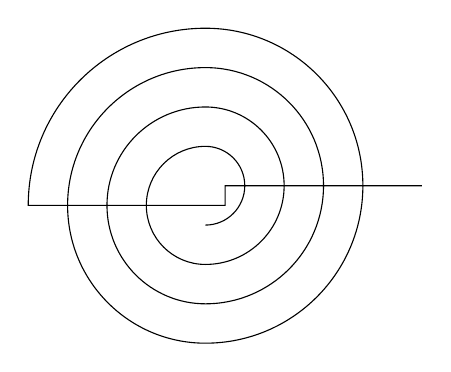
\begin{tikzpicture}
    \draw[spath/save global=spiral] 
    (5,0) -- (2.5,0) -- ++(0,-.25) -- ++(-2.5,0)
    arc[radius=2.25cm,start angle=180,end angle=90]
    arc[radius=2cm,start angle=90, delta angle=-180] 
    arc[radius=1.75cm,start angle=-90, delta angle=-180] 
    arc[radius=1.5cm,start angle=90, delta angle=-180] 
    arc[radius=1.25cm,start angle=-90, delta angle=-180] 
    arc[radius=1cm,start angle=90, delta angle=-180] 
    arc[radius=.75cm,start angle=-90, delta angle=-180] 
    arc[radius=.5cm,start angle=90, delta angle=-180]
    ;
    \end{tikzpicture}

\begin{tikzpicture} 
    \tikzset{
        spath/.cd,
        split at self intersections=spiral,
        get components of={spiral}\pathcomponents,
    }

    \foreach[count=\k] \cpt in \pathcomponents {
        \draw[spath/use=\cpt,-|];
        \node[fill=white, fill opacity=.5, circle, text opacity=1] at
        (spath cs:{\cpt} .5) {\(\k\)};
    }
\end{tikzpicture}

\begin{tikzpicture} 
    \tikzset{
        spath/.cd,
        split at self intersections=spiral,
        insert gaps after components={spiral}{10pt}{1,3,5,7,10,11,14}, 
        % 插入交点前后的间隔
        spot weld=spiral,
        get components of={spiral}\pathcomponents,
    }
    \foreach[count=\k] \cpt in \pathcomponents { 
        \draw[blue, line width=2pt,spath/use=\cpt];
    }
\end{tikzpicture}
\end{document}